\documentclass{article}
\usepackage[a4paper, margin=3mm, landscape]{geometry}
\usepackage{multicol}
\usepackage{xcolor}
\usepackage{enumitem}
\usepackage{amsmath}
\usepackage{amsfonts}
\usepackage{listings}
\usepackage{soul}
\usepackage{graphicx}

\pdfinfo{
    /Title (CS3219.pdf)
    /Creator (TeX)
    /Producer (pdfTeX 1.40.0)
    /Author (Jason Qiu)
    /Subject (CS3219)
    /Keywords (CS3219, nus, cheatsheet, pdf)
}

\graphicspath{ {./img/} }

\pagestyle{empty}
\setcounter{secnumdepth}{0}
\setlength{\columnseprule}{0.25pt}

% Redefine section commands to use less space
\makeatletter
\renewcommand{\section}{\@startsection{section}{1}{0mm}%
    {-1ex plus -.5ex minus -.2ex}%
    {0.5ex plus .2ex}%x
{\normalfont\large\bfseries}}
\renewcommand{\subsection}{\@startsection{subsection}{2}{0mm}%
    {-1explus -.5ex minus -.2ex}%
    {0.5ex plus .2ex}%
{\normalfont\normalsize\bfseries}}
\renewcommand{\subsubsection}{\@startsection{subsubsection}{3}{0mm}%
    {-1ex plus -.5ex minus -.2ex}%
    {1ex plus .2ex}%
{\normalfont\small\bfseries}}%
\makeatother

% Adjust spacing for all itemize/enumerate
\setlength{\leftmargini}{0.5cm}
\setlength{\leftmarginii}{0.5cm}
\setlist[itemize,1]{leftmargin=2mm,labelindent=1mm,labelsep=1mm}
\setlist[itemize,2]{leftmargin=2mm,labelindent=1mm,labelsep=1mm,label=$\bullet$}
\setlist[itemize,3]{leftmargin=2mm,labelindent=1mm,labelsep=1mm,label=$\bullet$}

% Font
\renewcommand{\familydefault}{\sfdefault}

% Define colors for math formulas
\definecolor{myblue}{cmyk}{1,.72,0,.38}
\everymath\expandafter{\the\everymath \color{myblue}}

% Custom command for keywords
\definecolor{highlight}{RGB}{251,243,218}
\newcommand{\keyword}[2]{\sethlcolor{highlight}\hl{\textbf{#1}} - #2}
\newcommand{\ilkeyword}[1]{\sethlcolor{highlight}\hl{\textbf{#1}}}

% Custom highlight colors
\definecolor{highlightgreen}{RGB}{134,241,212}
\definecolor{highlightorange}{RGB}{227,146,85}
\definecolor{highlightpurple}{RGB}{194,185,209}

% Custom command for partial derivatives
\newcommand{\partialderivative}[2][]{\frac{\partial #1}{\partial #2}}

% Define colors and style for code
\definecolor{codegreen}{rgb}{0,0.6,0}
\definecolor{codegray}{rgb}{0.5,0.5,0.5}
\definecolor{codered}{HTML}{CC241D}
\definecolor{backcolor}{rgb}{0.95,0.95,0.95}
\lstdefinestyle{codestyle}{
    backgroundcolor = \color{backcolor},
    commentstyle = \color{codegray},
    keywordstyle = \color{codered},
    stringstyle = \color{codegreen},
    basicstyle = \ttfamily,
    breakatwhitespace = false,
    showstringspaces = false,
    breaklines = true,
    showtabs = false,
    tabsize = 2
}
\lstset{style = codestyle}

% -----------------------------------------------------------------------
\begin{document}
\begin{multicols*}{4}
\footnotesize

% Title box
\begin{center}
    \fbox{
        \parbox{0.8\linewidth}{
            \centering \textcolor{black}{
                {\Large\textbf{CS3219}} \\
                \normalsize{AY24/25 Sem 1}} \\
                {\footnotesize \textcolor{gray}{github.com/jasonqiu212}}
        }
    }
\end{center}

\section{01. Introduction}

\subsection{Software Development Process}

\begin{itemize}
    \item \keyword{Waterfall}{Sequential approach good for stable req.}
    \item \keyword{Agile}{Iterative development with feedback loops and quick responses to changes}
    \begin{itemize}
        \item \keyword{Scrum}{Work done in sprints, where a subset of the product backlog is cleared}
    \end{itemize}
\end{itemize}

\subsection{Software Delivery}

\begin{itemize}
    \item \keyword{Deployment}{Make software available to use after dev.}
    \item \keyword{DevOps}{Practices combining software dev. and ops.}
    \begin{itemize}
        \item Purpose: Reduce time between committing change to the change reaching production while ensuring quality
        \item \keyword{Cont. Integration}{Auto build, unit test, deploy to staging, and acceptance test, to show problems early}
        \item \keyword{Continuous Delivery}{Same as above, except with manual deployment to production. Ensures that every good build is
        potentially ready for production release.}
        \item \keyword{Continuous Deployment}{Same as above, but with auto deployment to production}
    \end{itemize}
\end{itemize}

\section{02. Requirements}

\begin{itemize}
    \item Capabilities needed by user or must be met by system
\end{itemize}

\subsection{Requirement Types}

\begin{itemize}
    \item \keyword{Business Req.}{Why the organization is implementing the system, e.g., reduce staff costs by 25\%}
    \item \keyword{User Req.}{Goals the user must be able to perform with the prooduct, e.g., check for flight on website}
    \item \keyword{Functional Req. (FR)}{Specifies what a system does, e.g., website can export boarding pass}
    \item \keyword{Business Rules}{Policies that define or constrain requirements, e.g., staff gets 40\% discount}
    \item \keyword{Quality Attributes}{How well the system performs, e.g., Mean time bet. failure $\geq$ 100 hours. A type of non-functional req.}
    \item \keyword{System Req.}{Hardware or software issues, e.g., invoice system must share data with purchase order system}
    \item \keyword{External Interfaces}{Connections between systems and outside world, e.g., must import files in CSV format}
    \item \keyword{Constraints}{Limitations on implementation choices, e.g., must be backward compatible. Type of NFR.}
    \item Flow: Business Req. $\rightarrow$ \ilkeyword{Vision and Scope Document} $\rightarrow$ User Req. $\rightarrow$ \ilkeyword{User Req. Doc.} $\rightarrow$ FRs $\rightarrow$ SRS
\end{itemize}

\subsection{Requirements Development Phases}

\begin{itemize}
    \item \keyword{Elicitation}{Discover requirements (e.g., Interview)}
    \item \keyword{Analysis}{Analyze, decompose, derive, understand}
    \item \keyword{Specification}{Written or illustrated requirements}
    \item \keyword{Validation}{Confirm correct set of requirements}
    \item No linear path
\end{itemize}

\subsection{Requirements Development Outcomes}

\begin{itemize}
    \item \keyword{Software Req. Specification (SRS)}{Complete desc. of behavaior of software. Contains FRs, System Req., Quality Attributes, Ext. Interfaces, and Constraints.}
    \item \keyword{Rights, Responsibilities, and Agreements}{All stakeholders confident of development within balanced schedule, cost, functionality and quality}
    \item \keyword{Change Control}{Process to ensure changes to a product are introduced in a controlled and coordinated way}
\end{itemize}

\subsection{Quality Attributes}

\begin{itemize}
    \item Different apps have different quality attributes
    \item Quality attributes impact each other (Trade-offs)
    \item \keyword{Validation}{Do you have the right requirements?}
    \item \keyword{Verification}{Do you have the requirements right?}
\end{itemize}

\subsubsection{External}

\begin{itemize}
    \item Impacts user's experience
    \item \keyword{Safety}{Whether system can do harm}
    \item \keyword{Security}{Privacy, authentication, and integrity}
    \item \keyword{Performance}{Responsiveness of system. Impacts safety for real-time systems.}
    \item \keyword{Availability}{$\frac{\text{Up time}}{\text{Up time} + \text{Down time}}$}
    \item \keyword{Usability}{User-friendliness and ease of use}
    \item \keyword{Robustness}{How app performs when faced with invalid inputs, defects, and attacks}
    \item \keyword{Reliability}{Probability of app executing without failure}
    \item \keyword{Integrity}{Preventing information loss and preserving data correctness}
    \item \keyword{Interoperability}{How readily system can exchange data and services with other software and hardware}
    \item Others: Deployability, Compatibility, Installability
\end{itemize}

\subsubsection{Internal}

\begin{itemize}
    \item Perceived by developers and maintainers
    \item \keyword{Scalability}{Ability to have more users, servers, etc.}
    \begin{itemize}
        \item Vertical Scaling: Add capability of machines
        \item Horizontal Scaling: Add more machines
    \end{itemize}
    \item \keyword{Efficiency}{How well app uses hardware, network, etc.}
    \item \keyword{Modifiability}{How easily code can be understood, changed, and extended}
    \item \keyword{Portability}{Effort needed to migrate software from 1 environment to another}
    \item \keyword{Reusability}{Effort needed to convert software component for use in other apps}
    \item \keyword{Verifiability}{How well software can be evaluated to demonstrate that it functions as expected}
    \item Others: Maintainability, Testability
\end{itemize}

\section{03. Software Architecture}

\begin{itemize}
    \item Contains: Components, Connectors, Configuration
    \item \keyword{Reference Architecture}{Common architectural framework that leads to architectural patterns}
    \item \keyword{Control flow}{Connector indicating computation order}
    \item \keyword{Data flow}{Connector indicating data flow}
    \item \keyword{Call and return}{Control flow moves from 1 component to another and back}
    \item \keyword{Decomposition}{Breaking down a system}
    \begin{itemize}
        \item \keyword{Horizontal Slicing}{Designing by layers}
        \item \keyword{Vertical Slicing}{Designing by features}
        \item Criteria: Modularity, Coupling, Cohesion
    \end{itemize}
\end{itemize}

\subsection{Architectural Styles}

\begin{itemize}
    \item Categories: How is code divided? (Technical/domain partitioning), How is system deployed? (Monolithic, distributed)
    \item \keyword{Layered}{Software organized as layers of components}
    \item \keyword{Pipe and Filter}{Data flows through components (Data source, filters, data sink) via pipes}
    \item \keyword{MVC}{Model (Business logic), View, Controller (Coordinates between view and model)}
    \item \keyword{Web MVC}{2 communicating entities: Server (Holds the model) and Client (Interacts with the server)}
    \begin{itemize}
        \item Controller: Handles user HTTP request, selects model, prepares view
        \item Client-side Rendering (CSR): Rendered in browser with slower initial load but faster page changes
        \item Server-side Rendering (SSR): Rendered in server with faster initial load but requires more server resources
    \end{itemize}
    \item \keyword{Single Page App. (SPA)}{Implementation of CSR; retrieve data from server without refreshing single page}
\end{itemize}

\subsection{Representational State Transfer (REST)}

\begin{itemize}
    \item Set of rules for transferring, accessing, and manipulating textual data representations of hypermedia
    \begin{itemize}
        \item Not an architecture by itself
        \item \keyword{Hypermedia}{Combo. of multimedia and hyperlinks}
    \end{itemize}
    \item Client-server architecture: For separation of concerns
    \item Stateless: Interaction between client and server should contain all information for scalability and reliability
    \item Cacheable: Server response should include if data is caheable or not for network efficiency
    \item Layered: To reduce system complexity
    \item Uniform interface to interact with server (HTTP/S)
    \begin{itemize}
        \item Resource-based: Anything can be a resource
        \item Resources can be identified and manipulated by components (e.g., HTTP DELETE /user/:id)
    \end{itemize}
    \item Code-on-demand: Optional; Allow client functionality by downloading executable code
    \item Pros: Less coupled, scalability
    \item Cons: Being stateless decreases network performance
\end{itemize}

\section{04. Microservices Architecture}

\begin{itemize}
    \item \keyword{Microservices App.}{App. as suite of small services}
    \item Each microservice:
    \begin{itemize}
        \item has well-defined business capabilities
        \item has cohesive features
        \item is developed/deployed independently
        \item communicate with each other through well-defined mechanisms (Sync. or Async.)
    \end{itemize}
    \item How to identify boundaries of microservices? DDD and Event Storming
\end{itemize}

\subsection{Domain Driven Design}

\begin{itemize}
    \item \keyword{DDD}{Complex system is collection of multiple domain models (sub-domains)}
    \item \keyword{Domain}{Problem space that business occupies}
    \item \keyword{Sub-domain}{Component of main domain}
    \item \keyword{Bounded Context}{Cohesive boundary in the solution space relevant to the sub-domain that helps to define the models, functionalities, and implementation needed}
    \begin{itemize}
        \item Shared kernel: 2 contexts developed independently but overlaps (Tightly coupled teams)
        \item Upstream-downstream: 2 contexts in provider-consumer relationship through API
        \item Conformist relationship: Consumer conforms entirely to provider (Most loosely coupled between teams)
    \end{itemize}
    \item Interactions between contexts model interactions between sub-domains
    \item \keyword{Aggregate}{Cluster of related entities and value objects that are part of bounded context}
    \begin{itemize}
        \item Transactional boundary: Any change to aggregate will either all succeed or none will succeed
        \item Consistency boundary: Everything outside of aggregate can only read; state can only be modified through aggregate's public interface
        \item Aggregate Root: Aggregate's public interface
    \end{itemize}
\end{itemize}

\subsection{Event Storming}

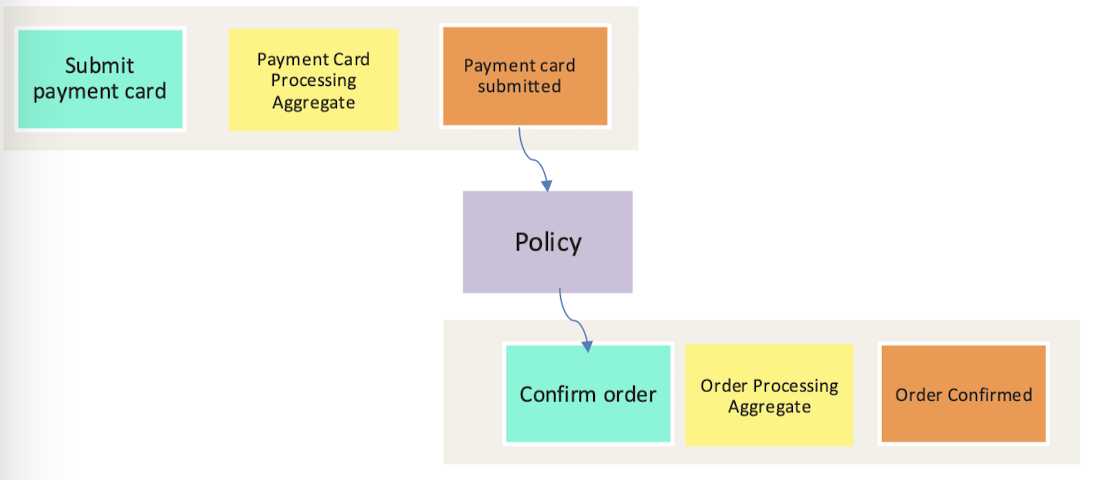
\includegraphics[scale=0.35]{event-storming.png}

\begin{itemize}
    \item \sethlcolor{highlightgreen}\hl{\textbf{Command}} - User or external action that causes events
    \item \keyword{Aggregate}{Unit for purpose of data changes after command and before event}
    \item \sethlcolor{highlightorange}\hl{\textbf{Domain events}} - Relevant events that occur in domain
    \item \sethlcolor{highlightpurple}\hl{\textbf{Policy}} - Relationship where event triggers command
    \item Bounded contexts determined by grouping commands, aggregates, and events, where policies link contexts
\end{itemize}

\subsection{Data Patterns in Microservices}

\begin{itemize}
    \item Motivation: How do microservices manage data?
    \item \keyword{Database-server-per-service Pattern}{Each service has its own database server}
    \begin{itemize}
        \item Data Indep.: Services should not modify same data
        \item Pros: Loose coupling, Easy interoperability
        \item Cons: Lots of DBs, Expensive
        \item Private-tables-per-service: Service owns private tables
        \item Schema-per-service: Service has private DB schema
    \end{itemize}
    \item \keyword{Delegate Pattern}{Access DB through authoritative delegate service and avoid accessing DB directly}
    \item \keyword{Data Lake Pattern}{Aggregate data from microservices into read-only, query-able data sinks}
    \item \keyword{Sagas Pattern}{All steps have a compensating action that's stored on routing slip and passed along}
    \begin{itemize}
        \item If step fails, roll back using routing slip and revert to \textbf{reasonably} compensated state (e.g. notification)
        \item For modifying data through multiple microservices
        \item Better for steps that are harder to compensate at end
    \end{itemize}
    \item \keyword{Event Sourcing}{Store stream of facts/events that got app. into current state, instead of storing current state}
    \begin{itemize}
        \item Different from relational/NoSQL
        \item Event: UUID, Event type, Data relevant to event type
        \item \keyword{Projection function}{Calculate new state using current state and new event}
        \item \keyword{Rolling snapshots}{Save projections to speed up perf.}
    \end{itemize}
    \item \keyword{Command Query Responsibility Segregation (CQRS)}{Split commands (write) from queries (read data)}
    \begin{itemize}
        \item E.g. commands write into Kafka queue of events; materialized view database derived from events
        \item Pros: Single write model can add data into many read models, Can scale independently
    \end{itemize}
\end{itemize}

\subsection{More Patterns in Microservices}

\begin{itemize}
    \item \keyword{Service Instance per Host}{Run each service instance in solation on its own host (e.g. VM, container)}
    \item \keyword{Immutable Infrastructure}{Component changes must be made by recreating component}
    \item \keyword{Infrastructure as Code}{Code can be easily versioned}
    \item \keyword{Orchestration}{Rely on central brain to drive processes}
    \item \keyword{Choreography}{Inform each component of its job, and let it work out the details}
    \item Service communication: Sync/async? 1-way or 2-way?
    \begin{itemize}
        \item \keyword{Event-Driven Communication}{See EDA}
        \item \keyword{Request-Response Communication}{"Do this"; Generally sync. (Latent and coupled)}
    \end{itemize}
    \item \keyword{API Gateway}{Entry point server that routes requests to services}
    \begin{itemize}
        \item Backends for Frontends: Gateway for each device type
    \end{itemize}
    \item \keyword{Service Discovery}{Service registry to store IP and port of each microservice}
    \begin{itemize}
        \item \keyword{Client-side Disc.}{Client determines location from registry and uses load-balancing to select}
        \item \keyword{Server-side Disc.}{Client req. to router/load balancer}
        \item \keyword{Service Registry Pattern}{Database of services and locations, where instances register with registry}
    \end{itemize}
\end{itemize}

\section{05. Scalability}

\begin{itemize}
    \item Strategies of scaling: Run multiple instances/copies, Split data, Split functionalities
    \item Scaling services in monolithic applications:
    \begin{itemize}
        \item \keyword{Scale Up}{Upgrade server}
        \item \keyword{Scale Out}{Run multiple instances}
        \begin{itemize}
            \item \keyword{Load Balancer}{Chooses service replica to execute user request}
            \item \keyword{Session Store}{Stores user's session across replicas}
        \end{itemize}
    \end{itemize}
    \item Scaling databases:
    \begin{itemize}
        \item \keyword{Caching}{Good for data that is frequently read and rarely changes}
        \item \keyword{Scaling Out with Read Replicas}{Write to primary and read from secondary to separate read and write}
        \item \keyword{Scaling Out by Partitioning Data}{Horizontal (By rows) vs. Vertical (By columns)}
        \item Scaling out databases creates \ilkeyword{distributed databases}
    \end{itemize}
    \item Scale multiple services to build multi-tiered apps.
    \item Split system into microservices to help scalability
    \item \keyword{Pod Architecture}{(Swim lanes) Place group of services/replicas inside boundary to contain failures}
\end{itemize}

\section{06. Event-Driven Architecture}

\begin{itemize}
    \item \keyword{Event}{Broadcasted to services that something \textbf{happened} and/or copies data to other services}
    \begin{itemize}
        \item \keyword{Initiating Event}{From end user}
        \item \keyword{Derived Event}{Created due to initiating event}
        \item Structure: Key-value pair (\keyword{Unkeyed}{No key}; \keyword{Entity}{Unique key}; \keyword{Keyed}{Key not unique; For partitioning})
        \item Publisher owns event payload and topic channel
    \end{itemize}
    \item \keyword{Event-Driven Architecture (EDA)}{\textbf{Event-based} with \textbf{async.} communication}
    \begin{itemize}
        \item \keyword{Real-time data}{Published as it is generated}
        \item Components: Producers, Brokers, Consumers
        \item Can combine into event-driven microservices 
        \item Pros: Fast since async., Scalable broker, Less coupled
    \end{itemize}
    \item \keyword{Broker}{Receives events, stores events in queue/partitions, and provides events for consumption (e.g., Kafka)}
    \begin{itemize}
        \item Properties: Immutable, Ordering, Indexing, Partitioning, Infinite retention, Replayability
        \item \keyword{Partition}{Indexed queue that \textbf{persists} after pop}
        \item Consumer consumes by index of last message it read
        \item \keyword{Topic}{Category of partitions; channel for \textbf{1-to-M} communication (Pub-Sub)}
        \begin{itemize}
            \item Multiple partitions $\rightarrow$ Non-sequential processing
        \end{itemize}
    \end{itemize}
\end{itemize}

\section{07. Asynchronous Communication}

\begin{itemize}
    \item Communication types: Sync./async.? Single/multiple receivers? Persistent/transient?
    \item \keyword{Synchronous}{Caller sends message and \textbf{waits} for receiver to respond with ack. (e.g., HTTP/S)}
    \item \keyword{Asynchronous}{Caller sends message and continues executing code without waiting (e.g., AMQP)}
    \begin{itemize}
        \item Pros: Available, Decoupling of sender and receiver
        \item Cons: More complex error-handling
    \end{itemize}
    \item \keyword{Message}{Carries \textbf{point-to-point} (1-to-1) command or data query to be executed by another service}
    \begin{itemize}
        \item vs. Event: Both for async. communication, but with different intent
        \item Receiver owns message payload and queue channel
    \end{itemize}
    \item \keyword{Queue}{FIFO channel with \textbf{single receiver} (P2P)}
    \begin{itemize}
        \item vs. Topic: Different intent and processing order
    \end{itemize}
    \item \keyword{Advanced Message Queueing Protocol (AMQP)}{P2P messaging protocol where client communicates with broker (e.g., RabbitMQ)}
    \begin{itemize}
        \item Messages published to \ilkeyword{exchanges}, which distribute message copies to queues
        \item Exchange types: Direct (Match), Fanout (All bounded queues), Topic (Wildcard match)
    \end{itemize}
    \item \keyword{Persistent}{Messages stored until next node receives}
    \item \keyword{Transient}{Messages only buffered for some time}
\end{itemize}

\section{08. Messaging Patterns}

\begin{itemize}
    \item Async. and enables enterprise integration
    \item Message contains: Header with message type, Payload
\end{itemize}

\subsubsection{Message Channel}

\begin{itemize}
    \item \keyword{Return Address}{Tells replier where to send reply to}
    \item \keyword{Correlation ID}{Specifies which request this reply is for}
    \item \keyword{Request-Reply Chaining}{Chain using correlation IDs}
    \item \keyword{Invalid Message Channel}{Handles erroneous messages}
    \item \keyword{Dead Letter Channel}{For failed-to-deliver messages}
    \item \keyword{Datatype Channel}{For specific type of data (RabbitMQ: Direct exchange chooses queue)}
    \item \keyword{Pub-Sub Request-Response Pattern}{Sender communicates with multiple services with Pub-Sub Channel (Topic), but all responses aggregated back using queue}
\end{itemize}

\subsubsection{Message Routing}

\begin{itemize}
    \item \keyword{Simple Router}{Routes 1 channel to many channels}
    \item \keyword{Composed Router}{Combination of routers}
    \item \ilkeyword{Context-Based Router} vs. \ilkeyword{Content-Based Router}
    \item \keyword{Msg. Filter}{Content-based router with 1 output channel (e.g., Pub-Sub Channel with filters)}
    \item \keyword{Msg. Splitter}{1 message $\rightarrow$ Multiple messages}
    \item \keyword{Msg. Aggregator}{Multiple correlated msgs. $\rightarrow$ 1 msg.}
    \item \keyword{Message Scatter-Gather}{Broadcasts 1 message to services and aggregates replies into single message}
\end{itemize}

\subsubsection{Message Transformation}

\begin{itemize}
    \item \keyword{Msg. Translator}{Converts msg. format}
    \item \keyword{Canonical Data Model}{Use common data format; requires 2 translators per service to translate in and out}
\end{itemize}

\subsubsection{Message Endpoint}

\begin{itemize}
    \item \keyword{Msg. Endpoint}{Interface bet. service and msg. system; channel-specific and distinct for send and receive}
    \item \keyword{Polling Consumer}{Service controls when to consume}
    \item \keyword{Event-Driven Consumer}{Consume on receive}
\end{itemize}

\section{09. Object Interaction Patterns}

\begin{itemize}
    \item \keyword{Design Pattern}{Solution to a problem in a context}
    \begin{itemize}
        \item Categories: Creational, Structural, Behavioral
    \end{itemize}
    \item \keyword{Data Transfer Object (DTO)}{Carries data between processes to reduce number of remote calls}
\end{itemize}

\subsection{Structural Design Patterns}

\begin{itemize}
    \item \keyword{Bridge}{Split large class into separate hierarchies of abstraction and implementation (e.g., Shape with color)}
    \item \keyword{Proxy}{Obj. sub. that controls access to original obj.}
    \item \keyword{Adapter}{Allows objects with incompatible interfaces to collaborate (Similar: Microservices, Msg. translator)}
    \item \keyword{Facade}{Provides simple unified interface to a set of subsystem interfaces (Similar: API Gateway)}
\end{itemize}

\subsection{Behavioral Design Patterns}

\begin{itemize}
    \item \keyword{Observer}{Subscription mechanism to notify observer objs. about events that happen to a subject obj.}
    \begin{itemize}
        \item Pull Model: Observer calls from subject when notified
        \item Push Model: Subject pushes snapshot on state change
    \end{itemize}
    \item \keyword{Mediator}{Forces objects to communicate via a mediator object (Similar: Event channel)}
\end{itemize}

\section{10. Principles}

\begin{itemize}
    \item \keyword{Modularity}{Independent modules that contains everything necessary to execute 1 functionality}
    \item \keyword{Single Resp. Prin. (SRP)}{Limit module to 1 purpose}
    \item \keyword{Sep. of Concerns}{Isolate distinct areas of functionality}
    \item \keyword{Loose Coupling}{Module knows little about others}
    \item \keyword{High Cohesion}{Bundle related behavior together}
    \item \keyword{Program to Interfaces}{Write code that depends on abstractions, rather than implementations}
    \item Information Hiding, Encapsulation
\end{itemize}

\end{multicols*}
\end{document}
